\documentclass[orivec]{llncs}

\usepackage{graphicx,url,wrapfig,amsmath,amssymb}

\usepackage[show]{ed} %for ednotes

\usepackage{macros/sembracket}
\usepackage{macros/mytikz}
\usepackage{macros/basics}
%\usepackage[llncs]{theorems} %only for now so that the environments are defined; replace with nice package for this later
\usepackage{local}

\usepackage{listings}

\lstdefinelanguage{mmt}{
	morekeywords={theory,namespace,rule,role,import,implicit,definitional,renaming},
	morecomment=[l][\color{Gray}]{//},
	% morecomment={[s]{//}{❚},[s]{//}{❙},[s]{//}{❘}}
}
\lstnewenvironment{mmtcode}[1][language=mmt]{\lstset{language=mmt,keywordstyle=\bfseries,basicstyle=\ttfamily,mathescape,columns=fixed,#1}}{}


\setcounter{tocdepth}{3}
\usepackage[bookmarks,linkcolor=red,citecolor=blue,urlcolor=gray,colorlinks,breaklinks,bookmarksopen,bookmarksnumbered]{hyperref}

\setlength{\hfuzz}{3pt}
\hbadness=10001 %make box warning less strict

\pagestyle{plain}

\begin{document}
\title{Structuring Theories with Implicit Morphisms}
\author{Florian Rabe$^{1,2}$ \and Dennis M\"uller$^2$}
\institute{LRI Paris \and FAU Erlangen-Nuremberg}
\maketitle

\begin{abstract}
We introduce \emph{implicit} morphisms as a concept in formal systems based on theories and theory morphisms.
The idea is that there may be at most one implicit morphism from a theory $S$ to a theory $T$, and if $S$-expressions are used in $T$ their semantics is obtained by automatically inserting the implicit morphism.
The practical appeal of implicit morphisms is that they hit the sweet-spot of being extremely simple to understand and implement while significantly helping with structuring large collections of theories.
\end{abstract}


\section{Introduction}
\paragraph{Motivation}
Theory morphisms have proved an essential tool for managing collections of theories in logics and related formal systems.
They can be used to structure theories and build large theories modularly from small components or to relate different theories to each other \cite{asl,devgraphs,littletheories}.
Areas in which tools based on theories and theory morphisms have been developed include specification \cite{obj,hets}, rewriting \cite{maude}, theorem proving \cite{imps,isabelle_locales}, and knowledge representation \cite{RK:mmt:10}.
Closely related concepts are used in both object-oriented (\emph{classes}) and functional (\emph{type classes}) programming languages.

%The latter of these tools is our \mmt system.
%We use \mmt as both a theoretical framework and a concrete implementation of our results.
%But our ideas are independent of \mmt and can be transferred very easily to any other language using theory morphisms.

These systems usually use a logic $L$ for the low-level formalization of domain knowledge, and a diagram $D$ in the category of $L$-theories and $L$-morphisms for the high-level structure of large bodies of knowledge.

\begin{wrapfigure}{r}{5.5cm}
\vspace{-3em}
\begin{tikzpicture}
\node (M) at (0,0) {$\cn{Monoid}$};
\node (G) at (-2,-2) {$\cn{Group}$};
\node (D) at (2,-2) {$\cn{DivGroup}$};
\draw[mono](M) -- (G);
\draw[arrow](G) to[out=30,in=150] node[above] {$\cn{G2DG}$} (D);
\draw[arrow](D) to[out=-150,in=-30] node[above] {$\cn{DG2G}$} (G);
\end{tikzpicture}
\vspace{-3.5em}
\end{wrapfigure}

For example, a document might reference an existing theory $\cn{Monoid}$, define a new theory $\cn{Group}$ that extends $\cn{Monoid}$, define a theory $\cn{DivGroup}$ (providing an alternative formulation of groups based on the division operation), and then define two theory morphisms $\cn{G2DG}:\cn{Group}\darr \cn{DivGroup}:\cn{DG2G}$ that witness an isomorphism between these theories.
This would result in the diagram on the right.%
\footnote{Note that we use the syntactic direction for the arrows, e.g., an arrow $m:S\to T$ states that any $S$-expression $E$ (e.g., a sort, term, formula, or proof) can be translated to a $T$-expression $m(E)$. Models are translated in the opposite direction.}
%Crucially, $m(-)$ preserves typing and provability.

The key idea behind implicit morphisms is very simple:
We maintain an additional diagram $I$, which is a commutative subdiagram of $D$ and whose morphisms we call \emph{implicit}.
The condition of commutativity guarantees that $I$ has at most one morphism $i$ from theory $S$ to theory $T$, in which case we write $\ipc{i}{S}{T}$.
Commutativity makes the following language extension well-defined: if $\ipc{i}{S}{T}$, then any identifier $c$ that is visible to $S$ may also be used in $T$-expressions, with the semantics being that $c$ abbreviates $i(c)$.
For example, in the diagram above, we may choose to label \cn{DG2G} implicit.
Immediately, every abbreviation or theorem that we have formulated in the theory \cn{DivGroup} becomes available for use in \cn{Group} without any syntactic overhead.
We can even label \cn{G2DG} implicit as well if we prove the isomorphism property to ensure that $I$ remains commutative, thus capturing the mathematical intuition that \cn{Group} and \cn{DivGroup} are just different formalizations of the same concept.
While these morphisms must be labeled manually, any inclusion morphism like the one from \cn{Monoid} to \cn{Group} can be made implicit automatically.

\paragraph{Contribution}
At the highest level, our contribution is the observation that implicit morphisms form a sweet spot of a very simple language feature that has substantial practical uses.
We recommend using implicit morphisms in all theory morphism--based formalisms.
More concretely, we present a formal system for developing structured theories with implicit morphisms.
Our starting point is the \mmt language \cite{RK:mmt:10}, which already provides a very general setting for defining and working with theories and morphisms.
\mmt is logic-independent, i.e., allows embedding a large variety of declarative languages (logics, type-theories, etc.).
Therefore, all our results can be directly applied to any language $L$ represented in \mmt or easily transferred to dedicated implementations of $L$.

We describe several example applications of implicit morphisms in detail: the identification of isomorphic theories, definitional extensions of theories, building large hierarchies of theories with many rarely used intermediate theories, seamlessly moving theories across logic morphisms, and transparently refactoring theory hierarchies.

\paragraph{Previous Work}
Implicit morphism were first conceived by Rabe in 2010 and implemented as part of the Twelf system \cite{twelf} (which implements the dependent type theory LF).
The theory behind this implementation was never written up and not published.
But the implementation already scaled well, and implicit morphisms were used in the LATIN logic atlas \cite{CHKMR:latinabs} built by Rabe and others in 2009--2012.
The LATIN atlas already has around a 1000 theories and atomic morphisms, and about 50 of the latter are marked as implicit.
It also has a few hundred inclusions, each of which induces another implicit morphism.

Since then, MMT has been developed, and
\begin{compactitem}
 \item implicit morphisms were generalized from LF to the logic-independent level of MMT,
 \item their theory was worked out,
 \item they were reimplemented from scratch as a part of MMT.
\end{compactitem}
MMT is backwards-compatible with Twelf, and the LATIN atlas including its implicit morphisms can be used from within MMT.
The present paper introduces these results in their final, most elegant form.

\paragraph{Overview}
In Sect.~\ref{sec:mmt}, we present the syntax and semantics of \mmt.
Even though the \mmt language is not new, our presentation is an entirely novel contribution in itself: it is much simpler and more elegant than the original one in \cite{RK:mmt:10}.
%Based on this extensible definition, we can introduce several additional structuring mechanisms.
%Many of these have already been implemented in the \mmt tool but were not formally defined --- a formal definition of their semantics as a part of the \mmt language had previously proved too complicated to spell out elegantly.
%With our reformulation, this is now not only possible but very easy.
%As an example, we define include declarations, the most important special case of implicit morphisms.
%\medskip
%
%Secondly, we describe implicit morphisms as a novel feature of \mmt.
Crucially, this increase in simplicity allows spelling out the syntax and semantics of implicit morphisms, which we do in Sect.~\ref{sec:impl}, within a few pages.
In Sect.~\ref{sec:appl}, we present applications.
Finally we discuss related and future work in Sect.~\ref{sec:conc}.

%In fact, implicit morphisms work so well that we have refactored the \mmt tool in such a way that implicit morphisms are now more primitive than inclusion morphisms.
%The semantics of inclusion morphisms is obtained by saying that inclusions are implicit morphisms that map all identifiers to themselves.
%Even the fundamental property that a theory may reference its own identifiers is then just a consequence of the fact that all identity morphisms are implicit.
%Therefore, surprisingly, adding the new feature of implicit morphisms to the \mmt kernel has made its design much simpler.


\section{Theories and Theory Morphism}\label{sec:mmt}
\subsection{Overview}

\begin{modexp}
\paragraph{Modularity in MMT}
As much as possible, theories and morphisms are treated uniformly, and we use the word \textbf{module} to refer to them collectively.
\mmt allows constructing large modules from small ones in two ways:
\begin{compactitem}
  \item \textbf{structured modules} contain declarations that import other, previously defined ones,
  \item \textbf{module expressions} are anonymous expressions (akin to formulas, terms, etc.) that denote modules.
\end{compactitem}

These two kinds of constructions have very different advantages but the same expressivity.
For example, we can construct the theory of commutative groups as the structured theory $\cn{CommutativeGroup}=\{\icl{Group},\icl{CommutativeMagma}\}$ or as the theory expression $\cn{Group}\cup\cn{CommutativeMagma}$.
The former is more practical when building named toplevel theories in software systems because each include is a separate declaration that can be parsed, checked, and flattened individually.
While negligible in this example, this becomes relevant quickly in large theories with complex structure.
The latter is more practical when building anonymous theory that are only needed temporarily.
In software systems, they also allow reusing operations like equality and $\lambda$-abstraction that already be implemented at the level of the base logic.
Building large morphism is as important as building large theories: for example, we want to be able to build morphisms out of $\cn{CommutativeGroup}$ by combining compatible morphisms out of $\cn{Group}$ and $\cn{CommutativeMagma}$.
\end{modexp}

\paragraph{Flat Modules}
\mmt provides formal syntax for both structured modules and module expressions and defines their semantics via \textbf{flattening}, which defines for every module $M$ a flat module $\flt{M}$.

\textbf{Flat theories} are lists of declarations $c:E[=e]$ where $E$ and $e$ are expression, and the latter is optional.
We write $\dom{T}$ for the set of constant identifiers $c$ in $\flt{T}$ and $\Exp{T}$ for the set of closed expressions using only the symbols $c\in\dom{T}$ (see below for the definition of well-formed expressions).
Constant declarations subsume virtually all basic declarations common in formal systems such as type/function/predicate symbols, axioms, theorems, inference rules, etc.
In particular, theorems can be represented via the propositions-as-types correspondence as declarations $c:F=P$, which establish theorem $F$ via proof $P$.
Similarly, \mmt expressions subsume virtually all objects common in formal systems such as terms, types, formulas, proofs.

Individual formal languages arise as fragments of \mmt: they single out the well-formed expressions by defining the two \mmt-\textbf{judgments} $\der_T e:e'$ (typing) and $\der_T e\equiv e'$ (equality) for every theory $T$ and $e,e'\in\Exp{T}$.
%This is already sufficient to define logical theorems as those formulas $F$ for which there is an object $p$ (the proof) such that $\der_T p:F$.
The details can be found in \cite{rabe:howto:14}.

\textbf{Flat morphisms} from a theory $S$ to a theory $T$ are lists of assignments $c:=e$ where $c\in\dom{S}$ and $e\in\Exp{T}$.
Every morphism $M$ induces a \textbf{homomorphic extension} $M(-):\Exp{S}\to\Exp{T}$, which replaces every $c\in\dom{S}$ in an $S$-expression with the $T$-expression $e$ such that $c:=e$ in $M$.

An \mmt \textbf{diagram} consists of a set of named structured module declarations.
\begin{nomodexp}
For a given diagram, we write $\Thy$ for the set of theory names.
And we write $\Mo{S}{T}$ for the set of morphisms defined by
\begin{compactitem}
 \item for every declaration $m:S\to T=\{\sigma\}$, we have $m\in\Mo{S}{T}$,
 \item for every $T\in\Thy$, we have $\id{T}\in\Mo{T}{T}$,
 \item for every $M\in\Mo{R}{S}$ and $N\in\Mo{S}{T}$, we have $M;N\in\Mo{R}{T}$.
\end{compactitem}
$\Thy$ and $\Mo{S}{T}$ form the category of theories and morphisms.
\end{nomodexp}
\begin{modexp}
Every diagram induces sets of anonymous module expressions.
These are mutually recursive: the names of the former provide the base cases for inductively forming the latter, and the latter may occur in the bodies of the former.
Every diagram induces sets
\begin{compactitem}
 \item $\thy$ of identifiers of theories $t$,
 \item $\Thy\supseteq \thy$ of theory expressions $T$,
 \item $\mo{S}{T}$ of identifiers of atomic morphisms $m$ from $S$ to $T$, and
 \item $\Mo{S}{T}\supseteq\mo{S}{T}$ of morphism expressions $M$ from $S$ to $T$.
\end{compactitem}
\end{modexp}
Then flattening assigns
\begin{compactitem}
 \item to each $T\in\Thy$ the flat theory $\flt{T}$,
 \item to each $M\in\Mo{S}{T}$ the flat morphism $\flt{M}$ from $\flt{S}$ to $\flt{T}$.
\end{compactitem}

\paragraph{Logics and Well-Formed Expressions}
The logic and the definition of well-formed expressions are not a primary interest of this paper, and we only recap the essential structure needed in the sequel.
We refer to \cite{rabe:howto:14} for details.

\mmt itself is independent of the base logic and provides a theory and theory morphism layer on top of an arbitrary declarative language.
Our results in this paper are similarly logic-independent.
The syntax and semantics of that base logic is provided by a set of rules for the judgments $\vdash_T e:E$ and $\vdash_T e=e'$ for $e,e',E\in\Exp{T}$.
The declarations in theories and morphisms are subject to typing conditions using these judgments.
The main theorem about \mmt is that well-typed morphisms $M:S\to T$ preserve all judgments, e.g,., if $\vdash_S e:E$, then $\vdash_T M(e):M(E)$.
This includes the preservation of truth via the propositions-as-types principle if $E$ is a proposition and $e$ its proof.

The only aspect of the inference system for these judgments that is relevant to our purposes here is the typing rule for constants:
\[\rul{c:E[=e] \minn \flt{T}}{\vdash_T c[=e]:E}\]
Here, in order to avoid case distinctions for the case where a definition is present or not, we use a combined typing+equality judgment: $e_1=e_2:E$ represents the conjunction of $e_1:E$, $e_2:E$, and $e_1=e_2$.
Correspondingly, the definition of the homomorphic extension of a morphism with domain $S$ includes the following case for constants:
\[M(c) = \cas{e\mifc (c:E) \in \flt{S}, (c:=e)\in\flt{M} \\ M(e) \mifc (c:E=e)\in \flt{S}}\]
Here if $c$ has a definiens in $S$, we expand it before applying $M$.%
\footnote{The \mmt tool accepts $c:e\in \flt{M}$ even if $(c:E=e')\in\flt{S}$ has a definition. In that case, \mmt checks $\vdash_T M(e')=e$ and puts $M(c)=e$. This is important for efficiency but not essential for our purposes here.}

Note that these base cases introduce a mutual recursion between well-formedness and flattening:
the well-formedness of a declaration in a theory depends on the flattening of all preceding declarations;
correspondingly, the well-formedness of an assignment in a morphism depends on the homomorphic extension of the morphism obtained by flattening of all preceding assignments.
Vice versa, well-formedness is a precondition for defining the flattening --- the definition of flattening may become nonsensical if applied to ill-formed modules.

It is desirable to define well-formedness independently of flattening.
But the mutual recursion makes sense from an implementation perspective: typical tools for formal systems first parse, check, and flatten a declaration entirely before moving on to the next declaration.
Moreover, often the checking of well-formedness is as difficult or expensive as flattening anyway.
In fact, inspecting practical systems with modular features (which often do not have a full rigorous formal specification) shows that our definition elegantly captures the essential commonalities between them.

Therefore, we will make flattening a partial function, i.e., $\flt{X}$ is undefined if the module $X$ is not well-formed. 

%Consider any declaration $n[:E][=e]$ in the body of a theory $t$.
%It is well-formed if $n$ is a fresh name $E$ and $e$ are well-formed expressions over $t$.
%(Additionally, $E$ and $e$ must satisfy typing conditions that are not essential for our purposes.)
%Importantly, $E$ and $e$ must be from $\Exp{\flt{t}}$ using only constants that were introduced in preceding declarations.
%
%Similarly, consider an assignment $c:=e$ in a morphism $m$ from $S$ to $T$, where $c:E$ is a declaration is $S$.
%It is well-formed if $\vdash_T e:\flt{m}(E)$.

\subsection{Syntax}

We start with the syntax for theories (which arises as a special case of the one given in \cite{RK:mmt:10}):

\begin{definition}[Theory]\label{def:theory}
The grammar for theories and expressions is of the form
\begin{grammar}
TDec     & T=\{Dec,\ldots,Dec\}  & \text{theory declaration} \\
Dec      & n:E\opt{=E}           & \text{constant declaration}\\
c        & t?n                   & \text{qualified constant identifiers} \\
E        & c \alt \ldots         & \text{expressions built from constants} \\
\end{grammar}

In a theory declaration, each symbol \textbf{name} $n$ may be declared only once, and its \textbf{type} and \textbf{definiens} (if present) must be closed expressions over the previously introduced constants only.
We omit the remaining productions for expressions here, which allow forming complex expressions using application, binding, variables, literals, etc.
\end{definition}

\begin{example}\label{ex:thgroup}
For the purposes of our running examples, we assume a fixed base logic that provides a first-order logic a simple type system.
\lstinline|type| is the universe of types, \lstinline|A ⟶ B| is the type of functions, and lambda abstraction is written \lstinline|[x:A] t x|.
We also use \mmt notations, which are attached to constant declarations as \lstinline|# <not>|; these are omitted from the formal grammar above because we only use them in the examples.

Then the (flat) theories $\cn{Group}$ and $\cn{DivGroup}$ from the introduction are:
\begin{mmtcode}
Group =
  U		: type
  op		: U ⟶ U ⟶ U	 # 1 ∘ 2 
  unit		: U
  inverse 	: U ⟶ U   # 1 ⁻¹ 
  // axioms omitted
\end{mmtcode}
\begin{mmtcode}
DivisionGroup =
  U 	: type
  div 	: U ⟶ U ⟶ U  # 1 / 2 
  unit 	: U
  // axioms omitted
\end{mmtcode}
\end{example}

At this point, this grammar only allows forming flat theories, i.e., $\Thy=\thy$.
It is intentionally independent of the concrete choice of modularity principles, i.e., the kinds of module-structuring declarations (e.g., includes) and the module-expression-forming operators (e.g., union).
But it already introduces all non-terminals for modularity: new declaration kinds for structured theories arise by adding productions for the non-terminal $Dec$ and new theory expressions are formed by adding productions for the non-terminal $T$.
This makes it easy to incrementally add new declaration kinds and operators to the language.

%These theories are similar to OpenMath content dictionaries \cite{openmath}.
%In particular, \mmt uses OpenMath-style qualified symbol identifiers $t?n$.%
%\footnote{Of course, the \mmt IDE and web interface parse and display these identifiers only as $n$ (if that is unambiguous), especially if they are used in formulas.
%But the interface always knows the qualified identifier and shows it, e.g., on hover.}
%Thus, symbols of the same name declared in different atomic theories are always distinguished.

We proceed accordingly for flat morphisms:

\begin{definition}[Morphism]\label{def:morphism}
A \textbf{morphism} is of the form
\begin{grammar}
MDec   & m:T\to T=\{Ass,\ldots,Ass\}     & \text{flat morphism declaration}\\
Ass    & c:=o                            & \text{assignment to symbol}\\
M      & m \alt \id{T} \alt M;M          & \text{morphism expressions}
\end{grammar}
such that a morphism declaration contains exactly one assignment $c:=o$ for each $c\in\dom{S}$, all of which satisfying $o\in\Exp{T}$.
\end{definition}

\begin{example}[Morphisms]\label{ex:dg2g}
We give the morphism \cn{DG2G} between the theories from Ex.~\ref{syn:incl}:
\begin{mmtcode}
DG2G : DivisionGroup -> Group =
  U 	:= U
  div 	:= [a,b] a ∘ (b⁻¹) 
  unit 	:= unit
  // assignments to axioms omitted
\end{mmtcode}
It maps the universe and unit of a division group to the corresponding notions of a group.
And we have $\cn{DG2G}(a/b)=a\circ b^{-1}$.
Additionally, the morphism must maps every axiom of \cn{DivGroup} to a proof in \cn{Group} of the translated statement, but we omit those assignments.
\end{example}

%Crucially, morphisms \textbf{preserve judgments}, in particular they map theorems to theorems.
%Formally, an atomic morphism $m:S\to T$ is \emph{well-formed} if
%\begin{compactitem}
%\item whenever $c$ has type $t$ in $\flt{S}$ and $c:= o$ in $\flt{m}$, then $\der_T o:m(t)$,
%\item whenever $c$ has definiens $d$ in $\flt{S}$ and $c:= o$ in $\flt{m}$, then $\der_T o\equiv m(d)$.
%\end{compactitem}
%Then we can show that for every $M\in\Mo{S}{T}$ if $\der_S o:o'$ (or $\der_S o\equiv o'$), then $\der_T M(o):M(o')$ (or $\der_T M(o)\equiv M(o')$).
%The details can be found in \cite{rabe:howto:14}.
%%In particular, this means that $M$ maps $S$-theorems to $T$-theorems.

Finally, we define diagrams as collections of modules:

\begin{definition}[Diagram]
A \textbf{diagram} is a list of theory and morphism declarations:
\begin{grammar}
Dia    & \rep{(TDec \alt MDec)}          & \text{diagrams}\\
\end{grammar}
A diagram is well-formed if each atomic theory/morphism declaration has a unique name and is well-formed relative to the diagram preceding it.
\end{definition}

We give some examples how to add modularity principles to the grammar:

\begin{example}[Includes]\label{syn:incl}
We extend the grammar with
\begin{grammar}
  Dec & \icl{S} & \text{include a theory into a theory} \\
  Ass & \icl{M} & \text{include a morphism into a morphism}
\end{grammar}
This allows writing the theory $\cn{Group}$ from Ex.~\ref{ex:thgroup} by extending a theory of monoids.
Again omitting all axioms, this looks as follows:
\begin{mmtcode}
Monoid =
  U 	: type
  op 	: U ⟶ U ⟶ U	 # 1 ∘ 2 
  unit	: U
Group =
  include Monoid
  inverse : U ⟶ U   # 1 ⁻¹ 
\end{mmtcode}
\end{example}

\begin{union}
\begin{example}[Union]\label{syn:union}
We extend the grammar with
\begin{grammar}
  T   & T\cup T & \text{union of theories} \\
  M   & M\cup M & \text{union of morphisms}
\end{grammar}
\end{example}
\end{union}

\begin{modexp}
\begin{example}[Category of Theories]\label{syn:cat}
To obtain the category structure of theories and morphisms, we need identity and composition.
We add them to the grammar as follows:
\begin{grammar}
  M   & \id{T} & \text{identity morphism} \\
  M   & M;M    & \text{morphism composition}
\end{grammar}
\end{example}
\end{modexp}

For each example, we will define the semantics in the next section.

\subsection{Semantics}

\paragraph{Flattening}
Just like the syntax, the definition of flattening is \textbf{compositional} in the sense that new modularity principles can be added later independently of each other.
In particular, for every module expression $X$, we define its flattening $\flt{X}$ by induction on the syntax.
This follows the principle of compositional semantics, e.g., $\flt{(f(X,Y))}$ depends only on $\flt{X}$ and $\flt{Y}$. 

For theories $T$, at this point, this induction only has the base case of a reference to a declared theory $t$.
Further cases arise when we add structuring declarations.

For the base case, of a theory $t=\{\Sigma\}$, we define $\flt{t}$ by induction on the declarations in $\Sigma$:
\[\flt{t}=\flt{\Sigma}\]
where
 \[\flt{\cdot}=\es\]
 \[\flt{(\Sigma,D)}=\flt{\Sigma}\cup\fltd{\flt{\Sigma}}{D}\]
Here $\fltd{T}{D}$ is the flattening of declaration $d$ relative to $\flt{\Sigma}$.

At this point, we only have one case for declarations $D$, namely constant declarations.
Their flattening is trivial:
 \[\fltd{\Sigma}{(n:E[=e])}=\{t?n:E[=e]\}\]
where $t$ is the name of the containing theory.

Correspondingly, for a declared morphism $m:S\to T=\{\sigma\}$, we have $m\in\Mo{S}{T}$ and $\flt{m}$ is defined by induction on the assignments in $\sigma$:
 \[\flt{\cdot}=\es\]
 \[\flt{(\sigma,\;A)}=\flt{\sigma}\cup\fltd{\flt{\sigma}}{A}\]
with the trivial base case
 \[\fltd{\sigma}{(c:=e)}=\{c:=e\}\]
\begin{nomodexp}
Moreover, for $T\in\Thy$ we define
\[\flt{\id{T}}=\{c:=c \;|\; c:E\in\flt{T}\}\]
And for $M;N\in\Mo{R}{T}$, we define
\[\flt{(M;N)}=\{c:=\flt{N}(\flt{M}(c)) \;|\; c:E\in\flt{R}\}\]
Note that in both cases, we only have to consider $R$-constants without definiens.
\end{nomodexp}

\begin{example}[Includes (continued from Ex.~\ref{syn:incl})]\label{sem:incl}
Includes add new declarations $D$, so we have to add cases to the definition of $\fltd{\Sigma}{D}$.
We do this as follows
  \[\fltd{\Sigma}{(\icl{S})} = \flt{S}\]
This has the effect of copying over all declarations from the included into the including theory.

Note that the definition of $\fltd{\Sigma}{n:E=e}$ qualifies the constant name $n$ with the theory name $t$ to form the identifier $t?n$ in the flattening.
Therefore, includes can never lead to name clashes.

Also note, that because $\flt{S}$ is a \textit{set} of declarations, the include relation is transitive: if $t$ includes $s$ via two different paths, $\flt{t}$ only contains one copy of the declarations of $\flt{s}$.
The situation is slightly more complicated for morphisms: if a morphism out of $t$ includes two different morphisms out of $s$, these have to agree.
Therefore, flattening and well-formedness must be distinguished:
  \[\fltd{\sigma}{(\icl{M})} = \flt{M}\]
under the condition $\flt{M}$ agrees with $\flt{\sigma}$ on any constant that is in the domain of both.

The flat variant $\cn{Group}^\flat$ of our refactored theory $\cn{Group}$ from Ex.~\ref{syn:incl} is hence given by copying all included symbols (from $\cn{Monoid}$) over to $\cn{Group}$, resulting in exactly the theory as presented earlier in \autoref{ex:thgroup} except for global identifiers from $\cn{Monoid}$ -- i.e. the prefixes $t$ in $t?n$.
\end{example}

\begin{union}
\begin{example}[Union (continued from Ex.~\ref{syn:union})]\label{sem:union}
We define the semantics of unions of theories as
\[\flt{(S\cup T)}=\flt{S}\cup\flt{T}\]
The handling of name clashes is the same as for includes:
Because the theories declared in a diagram have unique names and declarations in the flattening are qualified by theory names, union theories cannot have name clashes.
But we have to watch out when taking unions of morphisms:
We define $M_1\cup M_2\in \Mo{S_1\cup S_2}{T}$ if $M_i\in\Mo{S_i}{T}$ and $M_1$ and $M_2$ agree for every constant in $\dom{\flt{S_1}}\cap\dom{\flt{S_2}}$.
In that case, we put
\[\flt{(M\cup N)}=\flt{M}\cup\flt{N}\]
\end{example}
\end{union}

%Includes between theories are always well-formed (assuming the included theory is).
%But includes between morphisms are more difficult -- we have to impose two restrictions.
%Firstly, an assignment $\icl{M}$ is well-formed in an atomic morphism $m:S\to T$ if $R\harr S$ and $M\in\Mo{R}{T}$.
%Its intended effect is that $m$ maps all $c\in\dom{R}$ to $M(c)$.
%That yields the second restriction: For any two morphisms $M_i\in\Mo{R_i}{T}$ included into $m$ and any theory $C$ satisfying $C\harr R_1$ and $C\harr R_2$, we require that $M_1|_C\equiv M_2|_C$.
%Thus, any two included morphisms must agree on their common domain $C$; that is necessary so that $\flt{m}$ does not contain multiple assignments for the same identifier.

\begin{modexp}
\subsection{Semantic Properties}

For two theories $S,T\in\Thy$, we say that $S$ is \textbf{included} into $T$, written $S\harr T$, if $\flt{S}\sq\flt{T}$.
%Clearly, $m(o)=o$ for all $S$-objects $o$.
Thus, every declaration of $S$ is also available in $T$ and $\Exp{S}\sq\Exp{T}$.
This induces an inclusion morphism, which maps every $c\in\dom{S}$ to itself.
We do not introduce a name for that morphism and simply define $\id{S}\in\Mo{S}{T}$ whenever $S\harr T$ (which includes the special case $S=T$).
Moreover, if $S\harr T$ and $M\in\Mo{T}{U}$, we define the restriction $M|_S\in\Mo{S}{U}$ of $M$ to $S$ by $\id{S};M$.

We say that two theories $S,T\in\Thy$ are \textbf{equal}, written $S\equiv T$, if $\flt{S}=\flt{T}$.
This is equivalent to $S\harr T$ and $T\harr S$.

Correspondingly, we say that two morphisms $M,N\in\Mo{S}{T}$ are \textbf{equal}, written $M\equiv N$, if $\flt{M}=\flt{N}$.
In that case, $M(e)=N(e)$ for all expressions $e\in\Exp{S}$.

Clearly, $\equiv$ is an equivalence relation and $\harr$ is an order relation (if anti-symmetry is taken with respect to $\equiv$).

\begin{example}[Includes (continued from Ex.~\ref{sem:incl})]\label{rel:incl}
We have the following soundness theorem for includes: if a theory is declared as $t=\{\Sigma\}$ and $\Sigma$ contains $\icl{S}$, then $S\harr t$.

Note that in the absence of include declarations or unions, $s\harr t$ never holds because all $c\in\dom{s}$ are of the form $s?n$ and all $c\in\dom{t}$ are of the form $t?n$.
In fact, $\flt{s}$ and $\flt{t}$ unless $s=t$.
\end{example}

\begin{union}
\begin{example}[Union (continued from Ex.~\ref{sem:union})]\label{rel:union}
We have the following soundness theorem for unions: $S_i\harr S_1\cup S_2$.
Moreover, $S_1\cup S_2$ is a colimit in the category of theories and morphism, and given $M_1\in\Mo(S_1,T)$ and $M2\in\Mo{S_2,T}$ we have the universal morphism $M_1\cup M_2\in\Mo{S_1\cup S_2}{T}$ out of it.
\end{example}
\end{union}

\begin{example}[Category of Theories (continued from Ex.~\ref{sem:cat})]\label{rel:cat}
Identity and composition are congruent with respect to $\equiv$.
Moreover, composition is associative and identity neutral with respect to $\equiv$.
Thus, each diagram indeed yields the structure of a category with objects $\Thy$ and arrows $\Mo{S}{T}$.
\end{example}
\end{modexp}

%\section{Inclusion Morphisms}\label{sec:include}
%\subsection{Motivation}

\mmt as introduced in \cite{RK:mmt:10} allowed only two declarations in atomic theories: symbol declarations $c$ and structure declarations, which instantiate and import a theory.
(We omitted the latter in Sect.~\ref{sec:mmt}.)
We will now introduce include declarations to \mmt.

We can see include and structure declarations as duals.
Both import a previously declared theory, and both are transitive in the sense that if $T$ imports $S$, it also imports anything $S$ imports.
They differ in the sharing semantics when the same theory is imported multiple times: Multiple includes of $S$ are redundant and introduce a single copy of $S$; multiple structures of $S$ introduce multiple fresh copies of $S$.

Consequently, include declarations are \emph{unnamed} and the importing theory refers to the included symbols using the identifiers from $\dom{S}$.
Structure declarations on the other hand introduce a name in order to form qualified names for the fresh copy of the imported symbols.

\subsection{Definition}

We extend the \mmt grammar with
\begin{grammar}
  Dec & \icl{S} & \text{include a theory into an atomic theory} \\
  Ass & \icl{M} & \text{include a morphism into an atomic morphism}
\end{grammar}

We extend the definitions of $\flt{\Sigma}$ with the case
  \[\flt{(\Sigma,\;\icl{S})} = \flt{\Sigma}\cup\flt{S}\]
and the definition of $\flt{\sigma}$ with the case
  \[\flt{(\sigma,\;\icl{M})}=\flt{\sigma}\cup\flt{M}\]
%  \[\flt{(\Sigma,\;\strc{s}{S})} = \flt{\Sigma}\cup\{t?s/n[:t'][=d'] | n[:t][=d]\in \flt{S}\}\]
%where $t'$ and $d'$ arise from $t$ and $d$ by renaming all symbol identifiers accordingly.
%  \[\flt{(\sigma,\;\strca{M})}=\flt{\sigma}\cup\{t?s/n:=M(\flt{M}\]
In particular, this yields $S\harr t$ whenever $t$ declares an include of $S$.

Includes between theories are always well-formed (assuming the included theory is).
But includes between morphisms are more difficult -- we have to impose two restrictions.
Firstly, an assignment $\icl{M}$ is well-formed in an atomic morphism $m:S\to T$ if $R\harr S$ and $M\in\Mo{R}{T}$.
Its intended effect is that $m$ maps all $c\in\dom{R}$ to $M(c)$.
That yields the second restriction: For any two morphisms $M_i\in\Mo{R_i}{T}$ included into $m$ and any theory $C$ satisfying $C\harr R_1$ and $C\harr R_2$, we require that $M_1|_C\equiv M_2|_C$.
Thus, any two included morphisms must agree on their common domain $C$; that is necessary so that $\flt{m}$ does not contain multiple assignments for the same identifier.

\subsection{Discussion}

The original structure declarations of \mmt are significantly more expressive than include declarations: They allow fine-tuning the sharing by instantiating some symbols of the imported theory.
In particular, they can emulate include declarations as a special case.

But the inclusion relation $S\harr T$ induced by include declarations has a number of practically valuable properties.
Therefore, the author chose to add include declarations even though they do not adding expressive strength.
Indeed, the practical advantages are huge.
For example, after implementing support for inclusions, the author refactored the LATIN atlas \cite{CHKMR:latinabs:11} -- a large case study on formalizing logics using an \mmt style module system.
At this point it contains approximately $2000$ imports, of which $1600$ were changed to inclusions.
\medskip

There are several reasons for these advantages.
Firstly, inclusion is an order relation between theories: Each theory can be included at most once into another one.
That makes the inclusion relation very easy and efficient to maintain.

Secondly, we can form canonical qualified identifiers $s?n$ for identifiers of $s$ included into a theory $t$.
These are canonical identifiers that uniquely identify the included symbols and that are obvious to users.
Users can easily see where a symbol was imported from, but the import chain along which it was imported remains transparent.
%A qualified identifier $q.c$ where $q$ is provided by the import.
%This quickly leads to long names like $p.q.r.c$. Moreover, because the import path is part of the name, refactoring becomes more costly and multiple qualified identifiers may actually be the same.

Thirdly, $\Exp{s}\sq\Exp{t}$ so that the included declarations do not have to be translated from $s$ to $t$.
Consequently, implementations do not have to duplicate the translations: They can store all local declarations with the declaring theory, and use the relation $s\harr t$ to determine which theory may access which declarations.
Tools that duplicate imported declarations on the other hand quickly suffer from exponential blowups when handling large libraries.

Another advantage is that inclusion allows a form of implicit conversion.
As explained in \cite{RK:mmt:10}, we can consider morphisms $M\in\Mo{T}{F}$ as models of $T$ defined in terms of $F$.
For example, consider $T=\cn{Group}$ and $F=\cn{ZFC}$; then concrete group corresponds to morphisms $G\in\Mo{T}{F}$.
If we further assume $\cn{Monoid}\harr \cn{Group}$, then $G|_{\cn{Monoid}}$ is $G$ seen as a monoid.
Moreover, we can easily make the conversion $G\mapsto G|_{\cn{Monoid}}$ implicit without confusing humans or tools.
\medskip

Of course the above advantages are not a new discovery.
Many languages have long used a combination of unnamed and named imports (e.g., inheritance and aggregation in object-oriented programming correspond to includes and structures).
However, the above appears to be the first time that the semantics of include declarations is defined formally in the context of OpenMath-style qualified identifiers.

%\begin{compactitem}
%\item The original identifier $c$. This quickly leads to name clashes.
%\end{compactitem}
%There is one special case, where choosing identifies is easy: If $S\harr T$, e.g., $S$ is included into $T$.
%Then we can use $S.c$ as a qualified identifier.
%
%The reason why $S.c$ works as a qualified identifier is that $S$ can only be included into $T$ once and in a uniquely determined way.
%Implicit morphisms generalize this property: $S$ can only be implicitly mapped into $T$ once and in a that is uniquely determined by the implicit-diagram.
%Consequently, we can use any declaration $c$ of $S$ in $T$ using the identifier $S.c$.


\section{Implicit Morphisms}
\subsection{Overview}

Our key idea is to use a commutative subdiagram of the \mmt diagram, which we call the \emph{implicit-diagram}.
It contains all theories but only some of the morphisms --- the ones designated as \emph{implicit}.
Because the implicit-diagram commutes, there can be at most one implicit morphism from $S$ to $T$ --- if this morphism is $i$, we write $\ipc{i}{S}{T}$.
%Practically, this hasis a multi-graph whose nodes are the theories and whose edges are the atomic morphisms.
%We can extend the correspondence by identifying all paths with the composition of all edges along the path.
%Then concatenation of paths is just composition of morphisms, and the empty path from $T$ to itself is the identity morphism $\id{T}$.
%(This is well-defined because composition is associative and identity is neutral.)
%A diagram is commutative if any two paths between the same nodes are equal (with respect to $\equiv$), i.e., there is at most one morphism between any two nodes.
The implicit-diagram generalizes the inclusion relation:
All identity and inclusion morphisms are implicit, and we recover the inclusion relation $S\harr T$ as the special case $\ipc{\id{S}}{S}{T}$.
And just like inclusion, the relation ``exists $i$ such that $\ipc{i}{S}{T}$'' is a preorder.

Consequently, many of the advantages of inclusions carry over to implicit morphisms:
\begin{compactitem}
\item It is very easy to maintain the implicit-diagram, e.g., as a partial map that assigns to a pair of theories the implicit morphism between them (if any).
\item We can generalize the visibility of identifiers: If $\ipc{i}{S}{T}$, we can use all $S$-identifiers in $T$ as if $S$ were included into $T$.
Any $c\in\dom{S}$ is treated as a valid $T$-identifiers with definiens $M(c)$.
\item We can use canonical identifiers $S?n$ without worrying about ambiguity. Because there can be at most one implicit morphism $\ipc{i}{S}{T}$, using $S?n$ as an identifier in $T$ is unambiguous.
%Crucially, we can use $S?n$ without bothering what $i$ is.
\end{compactitem}

%Thus the main question arises what other morphisms we should make implicit.

\subsection{Syntax}

We introduce the family of sets $\IMo{S}{T}$ as a subset of $\Mo{S}{T}$, holding the \textit{implicit} morphisms.
The intuition is that $\Thy$ and $\IMo{S}{T}$ (up to equality of morphisms) form a thin broad subcategory of $\Thy$ and $\Mo{S}{T}$.

It remains to define which morphisms are implicit.
For that purpose, we allow \mmt declarations to carry \textit{attributes}:

\begin{definition}[Attributes for Implicitness]
We add the following productions
\begin{grammar}
MDec   & Att\; MDec  & \text{attributed morphism} \\
Dec    & Att\; Dec   & \text{attributed declaration}\\
Att    & \keyword{implicit} \alt \ldots & \text{attributes}
\end{grammar}
\end{definition}

The set of attributes is itself extensible, and the above grammar only lists the one that we use to get started.
Additional attributes can be added when adding modularity principles.

\begin{example}\label{ex:dg2gimplicit}
We can now change the declaration of the morphism $\cn{DG2G}$ from Ex.~\ref{ex:dg2g} by adding the attribute \keyword{implicit}.
\end{example}

\subsection{Semantics}

We only have to make two minor changes to the semantics to accommodate implicit morphisms.
The first change governs how we obtain implicit morphisms, the second one how we use them.

\begin{definition}[Obtaining Implicit Morphisms]
We define the set $\IMo{S}{T}\sq\Mo{S}{T}$ of \textbf{implicit} morphisms to contain the following elements:
\begin{itemize}
 \item all declared morphisms $m:S\to T=\{\sigma\}$ whose declaration carries the attribute $\keyword{implicit}$,
\begin{nomodexp}
 \item all identity morphisms $\id{T}$,
 \item all compositions $M;N$ of implicit morphisms $M$ and $N$,
\end{nomodexp}
 \item all morphisms that additional language features designate as implicit based on the use of additional attributes.
\end{itemize}

Adding an attribute to a declaration is only well-formed if there is (up to equality of morphisms) at most one implicit morphism for any pair of theories.
\end{definition}

\begin{modexp}
Depending on what modularity principles we add, equality of morphisms may or may not be decidable.
Therefore, in the general case, implementations may have to employ sound but incomplete criteria for equality (see Sect.~\ref{sec:commute}).
\end{modexp}

\begin{modexp}
The following example phrases the restriction on implicit morphisms in categorical terms:
\begin{example}[Category of Theories and Implicit Morphisms (continued from Ex.~\ref{sem:cat})]\label{impl:cat}
We define the following morphisms are implicit:
\begin{compactitem}
 \item all identity morphisms $\id{T}$,
 \item all compositions $M;N$ of implicit morphisms $M$ and $N$.
\end{compactitem}
Thus, the implicit morphisms form a thin broad subcategory of theories and morphisms.
In other words, the implicit morphisms form commutative diagram.
\end{example}
\end{modexp}

\begin{example}[Includes (continued from Ex.~\ref{sem:incl})]\label{impl:incl}
For include morphisms, we add the following definition: if theory $T$ contains the declaration $\icl{S}$, then the induced morphism from $S$ to $T$ is implicit.

Combined with composition morphisms, we see that all transitive includes between theories are implicit.
That corresponds to the intuition that anything that is included is available by its original name.
\end{example}

\begin{example}
	For our morphism $\cn{DG2G}$ from Ex.~\ref{ex:dg2gimplicit}, this means that all symbols declared in the theory $\cn{DivGroup}$ (see Ex.~\ref{ex:thgroup}) are now visible in the theory $\cn{Group}$ with the definitions provided by $\cn{DG2G}$.
	For example, we can write $a/b$ in $\cn{Group}$, where $/$ refers to the identifier $\cn{DivGroup}?\cn{div}$.
\end{example}

\begin{union}
It is plausible to say that there are implicit morphisms $S_i\harr S_1\cup S_2$ for $i=1,2$ that map all constants to themselves.
However, union expressions do not interact very well with implicit morphisms.
First of all, we have to be careful to maintain the uniqueness condition.
For example, assume there is a implicit morphism $M:S\to T$ that is not simply an inclusion.
Then the union $S\cup T$ cannot be well-formed.
If it were, we would have two different implicit morphisms $S\to S\cup T$, namely $M$ and the inclusion into the union.

Secondly, it becomes difficult to lookup whether an implicit morphism exists between union theories.
We need to consider the equational theory of union (including commutativity, idempotence, and associativity), which is doable for unions but may become undecidable if more module expression formation operators are added.
Already the interaction between union and composition morphisms can be tricky.

Therefore, we use the following definition in our system:

\begin{example}[Union (continued from Ex.~\ref{sem:union})]\label{impl:union}
We assume the definitions from Ex.~\ref{impl:cat} and~\ref{impl:incl} are in place.
We want to add union theories.
First of all, we note that every theory can be normalized into a union of named theories.

Now we make the following restriction on implicit morphisms: we maintain a diagram of implicit morphisms in which all nodes are \emph{named} theories, i.e., we do not allow implicit morphisms between union theories.
Because there are only finitely many named theories, this is a finite data structure.

Consequently, we have to forbid morphism declarations $\keyword{implicit}\,m:S\to T_1\cup T_2$ is a union --- there would be no way to record them in our diagram.
We can allow declarations declarations $\keyword{implicit}\,m:s_1\cup\ldots\cup s_n\to t$ where the domain is a union of named theories --- in that case we simply record $m$ as an implicit morphism from $s_i$ to $t$ for all $i$.
Similarly, any declaration $\icl{s_1\cup\ldots\cup s_n}$ in the body of theory $t$ poses no problems --- we record inclusion morphism $s_1\harr t$.

Now to look up the implicit morphism (if any) from $s_1\cup\ldots\cup s_k\to t_1\cup\ldots\cup t_l$, we look up for every $i$ an implicit morphism $m_i:s_i\to t_j$ for some $j$.
If all these $m_i$ exist and $m=m_1\cup \ldots\cup m_k$ is well-formed, then $m$ is the needed implicit morphism.
\end{example}
\end{union}

The intuition behind implicit morphisms is that all $S$-constants $c:E$ that can be mapped into the current theory via an implicit morphism $M:S\to T$ are directly available in $T$.
We can practically realize this by adding new defined constants $c:M(E)=M(c)$ to $T$.
However, physically adding definitions can be inefficient.
It is more elegant to modify the typing rules such that $\vdash_T c:M(c)=M(E)$ holds without any changes to $T$.

To do that, we only have to make a small modification to the original rules of \mmt as presented in Sect.~\ref{sec:mmt}.
To illustrate how simple the modification is, the following definition repeat the original rule first for comparison:

\begin{definition}[Using Implicit Morphisms]\label{def:useimpl}
We replace the rule
\[\rul{c:E[=e] \minn \flt{T}}{\vdash_T c[=e]:E} \tb \mwith\tb \rul{c:E[=e] \minn \flt{S}\tb \ipc{M}{S}{T}}{\vdash_T c=M(c):M(E)}\]
\end{definition}

Note that the modified rule gives every constant a definiens.
This is a technical trick to subsume the original rule: if $c$ is already declared in $T$, we use $M=\id{T}$ and obtain $\vdash_T c=c:E$.

The following theorem is our central theoretical result.
It shows that the modification made in Def.~\ref{def:useimpl} has the intended properties:
\begin{theorem}[Conservativity of Implicit Morphisms]
For well-formed diagrams and $S,T\in\Thy$ and $M\in\Mo{S}{T}$:
\begin{compactenum}
 \item Whenever the original system proves $\vdash_T e=e':E$, so does the modified one.
 \item Whenever the modified system proves $\vdash_T e=e':E$, then the original system proves $\vdash_T \ov{e}=\ov{e'}:\ov{E}$.
\end{compactenum}
Here $\ov{E}$ is the expression that arises from $E$ by recursively replacing every constant with its definiens.
\end{theorem}

\begin{proof}
For the first claim, we proceed by induction on derivations.
We only need to consider the case where the original rule was applied.
So assume it yields $\vdash_T c[=e]:E$, i.e., $(c:E[=e]) \minn \flt{T}$.
We apply the modified rule for the special case $\ipc{\id{T}}{T}{T}$.
The conclusion reduces to
\begin{compactitem}
 \item if $e$ is absent: $\vdash_T c=c:E$, which is equivalent to $\vdash_T c:E$,
 \item if $e$ is present: $\vdash_T c=e:E$ because $M(c)=M(e)$ according to the definition of $M(-)$.
\end{compactitem}

For the second claim, we proceed by induction on derivations.
We only need to consider the case where the modified rule was applied.
So assume it yields $\vdash_T c=M(c):M(E)$ for $(c:E[=e]) \minn \flt{S}$ and $\ipc{M}{S}{T}$.
We distinguish two cases:
\begin{compactitem}
 \item $M(c)=c$, i.e., $e$ is absent, and $\ov{c}=c$.
   According to the definition of $\flt{S}$, this is only possible if $S\harr T$ (including the special case $S=T$).
   In that case, $\flt{S}\sq\flt{T}$ and $M$ is the include/identity morphism that maps all $S$-constants to themselves.
   Now applying the induction hypothesis to the well-formedness derivation of $E$ yields $\vdash_T c:\ov{E}$ as needed.
 \item $M(c)\neq c$, i.e., $e$ is present or $M$ assigns a non-trivial value to $c$.
  Definition expansion eliminates $c$ in favor of $M(c)$, and thus $\ov{c}=\ov{M(c)}$.
  We only have to show that $\vdash_T \ov{M(c)}:\ov{M(E)}$ That follows from the judgment preservation of morphisms.
\end{compactitem}
\end{proof}

%\subsection{Commutativity}\label{sec:commute}
%
%To prove commutativity, we have to find all paths in the implicit-diagram and check $M\equiv M'$ for all pairs of morphisms between the same nodes.
%
%\mmt reduces $M\equiv M'$ for $M,M'\in\Mo{S}{T}$ to a first-order problem in the theory of categories, which uses the following axioms:
%\begin{compactitem}
%\item associativity of composition,
%\item neutrality of identity,
%\item $M;M'\equiv \id{S}$ as well as $M';M\equiv\id{T}$ if $M\in\Mo{S}{T}$ and $M'$ is the known *inverse of $M$,
%\item if an atomic morphism $m$ includes $M\in\Mo{R}{T}$, then $M|_R\equiv M$.
%\end{compactitem}
%
%This is a sound but not complete axiomatization of $M\equiv M'$.
%We can obtain a complete axiomatization in a totally different way: Check $\der_T M(c)\equiv M'(c)$ for all $c\in\dom{S}$.
%However, this can be extremely expensive: It requires computing $\dom{S}$ and proving an object level equality for each identifier.
%Even if the equality of objects is decidable, this is often too expensive.
%
%In fact, because implicit morphisms are meant to be used in very particular cases, we expect the above incomplete calculus to perform reasonably well in practice.
%If showing the equality of certain morphisms is hard, one should probably not make them implicit in the first place.



\section{Applications}
\subsection{Identifying Theories via Implicit Isomorphisms}\label{sec:inverse}

In this section, we introduce several language extensions that introduce implicit isomorphisms.

Note that because identity morphisms are implicit, our uniqueness requirement for implicit morphisms implies that two theories $S$ and $T$ must be isomorphic if there are implicit morphisms in both directions.
Moreover, making a pair of isomorphisms implicit is well-formed if there are no other implicit morphisms between $S$ and $T$ yet.

\paragraph{Renamings}
We say that a named morphism $r:S\to T=\{\ldots\}$ is a \textbf{renaming} if
\begin{compactitem}
 \item all assignments in its body are of the form $c:=c'$ for $T$-constants $c'$ without definiens
 \item every such $T$-constants $c'$ occurs in exactly one assignment.
\end{compactitem}
Clearly, every renaming is an isomorphism.
The inverse morphisms contains the flipped assignments $c':=c$.

We make the following extension to syntax and semantics:
\begin{compactitem}
  \item A morphism declaration $r:s\to t=\{\ldots\}$ may carry the attribute \keyword{renaming}.
  \item This is well-formed if there are no implicit morphism between $s$ and $t$ yet.
  \item In that case, we define $r\in\IMo{s}{t}$ and $r^{-1}\in\Mo{t}{s}$.
\end{compactitem}

\begin{example}
	Consider a variation of the theory $\cn{Monoid}$ from \autoref{syn:incl} in a different library:
	\begin{mmtcode}
Monoid2 =
  M: type
  connective : M ⟶ M ⟶ M	 # 1 ∘ 2 
  neutral	: M
\end{mmtcode}
This theory is isomorphic to the previously introduced theory $\cn{Monoid}$ under the trivial renaming
	\begin{mmtcode}
Monoids : Monoid2 -> Monoid =
  M 		:= U
  connective 	:= op 
  neutral	:= unit
\end{mmtcode}
\end{example}

\paragraph{Definitional Extensions}
We say that the named theory $t$ is a \textbf{definitional extension} of $S$ if $t=S$ or the body of $t$ contains
\begin{compactitem}
 \item only constant declarations with definiens,
 \item only include declarations of theories that are definitional extensions of $S$.
\end{compactitem}
\begin{example}
	Imagine extending the theory $\cn{Group}$ from \autoref{syn:incl} by provable theorems:
		\begin{mmtcode}
Group_Theorems =
  include Group
  inverse_idem : ⊦∀[x] (x⁻¹)⁻¹≐x 	= (proof)
\end{mmtcode}
\end{example}

If $t$ is a definitional extension of $S$, it is easy to prove that $t$ and $S$ are isomorphic: both isomorphisms map all constants without definiens to themselves. In particular, the isomorphism $S\to t$ maps $S$-constants to themselves and expands the definiens of all other constants.

We make the following extension to syntax and semantics:
\begin{compactitem}
  \item An include declaration $\icl{s}$ of a named theory $s$ inside theory $t$ may carry the attribute \keyword{definitional}.
  \item In that case, we define $\id{s}\in\IMo{t}{s}$ (in addition to the implicit morphism $\id{t}\in\IMo{s}{t}$ which is induced by the inclusion).
\end{compactitem}
\begin{example}
	We adapt our theory $\cn{Group\_Theorems}$ with the newly introduced keyword, which allows us to extend $\cn{Group}$ directly while having the new theorem $\cn{inverse\_idem}$ available:
		\begin{mmtcode}
Group_Theorems =
  definitional include Group
  inverse_idem : ⊦∀[x] (x⁻¹)⁻¹≐x 	= (proof)

More_Theorems =
  include ?Group
  some_other_theorem : ⊦ ??	= (proof using inverse_idem)
\end{mmtcode}
\end{example}

\begin{remark}[Conservative Extensions]
A definitional extension is a special case of a conservative extension.
More generally, all retractable extensions are conservative, i.e., all extensions $S\harr T$ such that there is a morphism $r:T\to S$ such that $r$ is the identity on $S$.

But we cannot make the retractions implicit morphisms in general because they are not necessarily isomorphisms.
\end{remark}

\paragraph{Canonical Isomorphisms}
If we have isomorphisms $m:s\to t$ and $n:t\to s$, we simply spell them out in morphism declarations and add the keyword \keyword{implicit} to both.
This requires no language extensions.

\begin{example}\label{group:iso}
Having declared the morphism $\cn{DG2G}$ (as in \autoref{ex:dg2g}) implicit, we do the same with the reverse morphism  $\cn{G2DG}$:
\begin{mmtcode}
implicit G2DG : Group -> DivisionGroup =
  U := U
  op := [a,b] a / ((unit/unit) / b) 
  unit := unit/unit
  inverse := [a] (unit/unit) / a
\end{mmtcode}
\end{example}

While the first one of these isomorphism declarations is straightforward, the second one requires checking that $m$ and $n$ are actually isomorphisms.
Otherwise, the uniqueness condition would be violated.
Thus, we have to check $m;n=\id{s}$ and $n;m=\id{t}$.
In general, the equality of two morphisms $f,g:A\to B$ is equivalent to $\vdash_B f(c)=g(c)$ for all $c:E\in\flt{A}$.
Thus, if equality of expressions is decidable in the logic that \mmt is instantiated with, then \mmt can check this directly.

However, this does not work in practice.
Already elementary examples require stronger, undecidable equality relations are used:

\begin{example}
Consider the isomorphism from Ex.~\ref{group:iso}.
The result of mapping $x\circ y$ from $\cn{Group}$ to $\cn{DivGroup}$ and back is $x\circ(unit\circ y^{-1})^{-1}$.
Clearly, the group axioms imply that this is equal to $x\circ y$.
But formally that requires working with the undecidable equality of first-order logic.
\end{example}

Therefore, in our running example, we only make one of the two isomorphisms implicit.

In the sequel, we design a general solution to this problem.
It allows systematically proving the equality of two morphisms and using that to make both isomorphisms implicit.
This is novel work, but it requires significant prerequisites and is only peripherally related to implicit morphisms.
Therefore, we only sketch the idea and leave the details to future work.

We add a language feature to \mmt to prove equalities between morphisms:
We add the productions
\begin{grammar}
Dia   & \rep{(TDec \alt MDec\alt MEq)}  &\\
MEq   & \keyword{equal} M=M:T\to T by \{\rep{Ass}\} &\\
\end{grammar}

%Firstly, the intuition of $\keyword{equality} T = \{c:=E,\ldots\}$ is that it provides to every base type $c:\type$ of $T$ a judgment $E:c\to c\to \type$ that defines the $T$-specific equality relation for objects of type $c$.
%Technically, this must be a binary logical relation in the sense of \cite{RS:logrels:12} on $\id{T}$.
%As described in \cite{RS:logrels:12}, this induces an equality predicate $\cn{Equal}_E:E\to E\to \type$ on every type $E$.

We define the declaration $M=N:S\to T by \{\sigma\}$ to be well-formed iff
\begin{compactitem} 
  \item $M:S\to T$ and $N:S\to T$ are well-formed morphisms
  \item $\sigma$ contains exactly one assignment $c:=p$ for every $(c:E)\in\flt{S}$
  \item for each of these assignments $c:=p$, the term $p$ is a proof of $\vdash_T M(c)=N(c)$.
\end{compactitem}

To make $m$ and $n$ from above implicit isomorphisms, we have to do three things: define $m$ and $n$, prove the equalities of $m;n=\id{s}$ and $n;m=\id{t}$, and make $m$ and $n$ implicit.
Note that we cannot make both $m$ and $n$ implicit right away because that is only well-formed after proving the equalities.)
Thus, we define a new attribute \keyword{implicit-later}, which states that a morphism should be considered implicit as soon as subsequent equality proves make it well-formed to do so.

\begin{example}[Isomorphisms]
We can now add declarations
 \[\keyword{implicit}:\cn{DG2G}:\cn{DivGroup}\to\cn{Group}=\text{(as above)}\]
 \[\keyword{implicit-later}:\cn{G2DG}:\cn{Group}\to\cn{DivGroup}=\text{(as above)}\]
 \[\keyword{equal}\cn{G2DG};\cn{DG2G}=\id{\cn{Group}}:\cn{Group}\to\cn{Group}=\text{(omitted)}\]
 \[\keyword{equal}\cn{DG2D};\cn{G2DG}=\id{\cn{DivGroup}}:\cn{DivGroup}\to\cn{DivGroup}=\text{(omitted)}\]
where the isomorphisms are as above and we omit all the equality proofs.
\end{example}

\subsection{Fine-Granular and Flexible Theory Hierarchies}
A common problem when defining modular theory hierarchies is that the most natural include-hierarchy for the most important theories is not necessarily the same as the most comprehensive hierarchy.
For example, Ex.~\ref{syn:incl} defines \cn{Group} with an include from \cn{Monoid}.
Instead, we could include \cn{Monoid} into the intermediate theory \cn{CancellationMonoid} and include that into \cn{Group}.
This change is not possible in retrospect --- changing the theory hierarchy (which is one of the most fundamental structures of a library) usually presents an insurmountable refactoring problem.
So instead we could systematically build a hierarchy that uses every intermediate theory (as done in \cite{mathscheme}).
But this yields a very deep and complex hierarchy that is hard to navigate for casual users.
Moreover, it does not protect us from later on discovering yet another intermediate theory that should have been added.

Implicit morphisms provide a simple solution to this problem because they behave effectively like inclusions but can be added later on.
In the above example, we would
\begin{compactitem}
 \item define \cn{CancellationMonoid} with an include from \cn{Monoid},
 \item keep \cn{Group} as it is, i.e., also with an include \cn{Monoid},
 \item add an implicit morphism $\cn{CancellationMonoid}\to\cn{Group}$.
\end{compactitem}
\medskip

As a more complex example, we have built a hierarchy of theories between \cn{Band} and \cn{Semilattice}.
\ednote{@DM: this is not quite the lattice from the Wikipedia page: it consists of the 3x3 square plus Bands at the top}
All of these theories are of the form $t=\{\icl{\cn{Band}},\,a:\vdash F\}$, where $F$ is a universally quantified equational axiom.\footnote{All varieties of bands can be axiomatized in this way.}
In particular, $\cn{SemiLattice}=\{\icl{\cn{Band}},\,a:\vdash \forall [x]\forall [y] x\circ y\doteq y\circ x\}$.
Fig.~\ref{fig:bands} shows these theories.

There are various morphisms between them that describe the lattice structure of the corresponding varieties of bands.
All of these map the constants from \cn{Band} to themselves and the axiom $a$ to a proof.%
\footnote{Our formalization of the lattice of bands using implicit morphisms can be found at \url{https://gl.mathhub.info/MitM/smglom/blob/devel/source/algebra/bands.mmt}.}
We make all of these morphisms implicit.
It is straightforward to prove that the diagram commutes: any two morphisms are identical except for assignment for the axiom.
Here, \mmt can discharge the proof obligation easily using proof irrelevance.

\begin{figure}\begin{center}
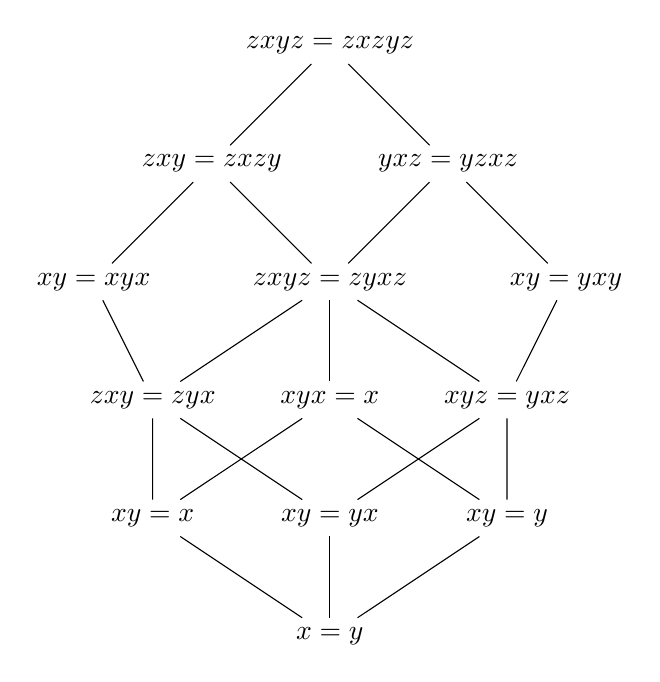
\begin{tikzpicture}[scale=1.5]
  \node (s1) at (0,0) {$zxyz=zxzyz$};
  
  \node (s2a) at (-1,-1) {$zxy=zxzy$};
  \node (s2b) at (1,-1) {$yxz=yzxz$};
  \draw (s1) to (s2a) {};
  \draw (s1) to (s2b) {};
  
  \node (s3a) at (-2,-2) {$xy=xyx$};
  \node (s3b) at (0,-2) {$zxyz=zyxz$};
  \node (s3c) at (2,-2) {$xy=yxy$};
  \draw (s2a) to (s3a) {};
  \draw (s2a) to (s3b) {};
  \draw (s2b) to (s3b) {};
  \draw (s2b) to (s3c) {};
  
  \node (s4a) at (-1.5,-3) {$zxy=zyx$};
  \node (s4b) at (0,-3) {$xyx=x$};
  \node (s4c) at (1.5,-3) {$xyz=yxz$};
  \draw (s3a) to (s4a) {};
  \draw (s3b) to (s4a) {};
  \draw (s3b) to (s4b) {};
  \draw (s3b) to (s4c) {};
  \draw (s3c) to (s4c) {};
  
  
  \node (s5a) at (-1.5,-4) {$xy=x$};
  \node (s5b) at (0,-4) {$xy=yx$};
  \node (s5c) at (1.5,-4) {$xy=y$};
  \draw (s4a) to (s5a) {};
  \draw (s4a) to (s5b) {};
  \draw (s4b) to (s5a) {};
  \draw (s4b) to (s5c) {};
  \draw (s4c) to (s5b) {};
  \draw (s4c) to (s5c) {};
  
  \node (s6) at (0,-5) {$x=y$};
  \draw (s5a) to (s6) {};
  \draw (s5b) to (s6) {};
  \draw (s5c) to (s6) {};
  
  %\node[thy,inner sep=.3cm,fill=gray] (t1) at (0,0) {};
  %\node at (t1.north west) {$S$};
  %\node at (t1) {$D$};
  %\node[thy,inner sep=.5cm,fill=lightgray] (s2) at (2,0) {};
  %\node[thy,inner sep=.3cm,fill=gray] (t2) at (2,0) {};
  %\node at (t2.north west) {$T$};
  %\node at (t2) {$C$};
  %\draw[view] (t1) to[out=10,in=170] node[above] {$\sigma$} (t2);
\end{tikzpicture}

%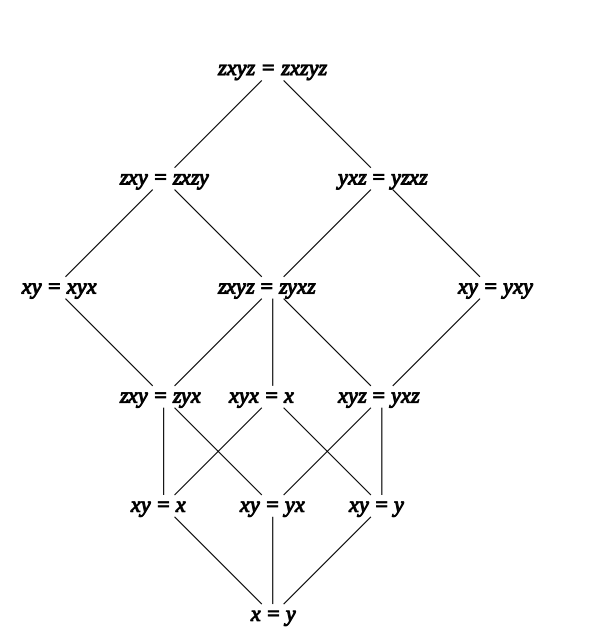
\includegraphics[width=0.6\textwidth]{bands}
\end{center}
\caption{The Lattice of Varieties of Bands}\label{fig:bands}
\end{figure}

%
%\begin{figure}
%\begin{tabular}{c|c}
%\begin{mmtcode}
%Band =
%  include ?SemiGroup
%  axiom_idemp : ⊦ ∀[x] x ∘ x ≐ x
%❚
%
%Regular =
%  include ?Band
%  axiom_regular : ⊦ ∀[x]∀[y]∀[z] 
%    z ∘ x ∘ z ∘ y ∘ z ≐ z ∘ x ∘ y ∘ z
%❚
%
%LeftNormal =
%  include ?Band
%  axiom_leftnormal : ⊦ ∀[x]∀[y]∀[z] 
%    z ∘ x ∘ z ∘ y ≐ z ∘ x ∘ y
%
%theory RightNormal =
%  include ?Band ❙
%  axiom_rightnormal : ⊦ ∀[x]∀[y]∀[z] 
%    y ∘ z ∘ x ∘ z ≐ y ∘ x ∘ z ❙ 
%❚
%
%theory Normal : ?Meta =
%  include ?Band ❙
%  axiom_normal :  ⊦ ∀[x]∀[y]∀[z] 
%    z ∘ x ∘ y ∘ z ≐ z ∘ y ∘ x ∘ z ❙
%❚
%\end{mmtcode} &
%\begin{mmtcode}
%implicit view Reg2LeftNormal : 
%    ?Regular -> ?LeftNormal =
%  include ?Band = ?Band ❙
%  axiom_regular = sketch "trivial" ❙
%❚
%
%implicit view Reg2RightNormal : 
%    ?Regular -> ?RightNormal =
%  include ?Band = ?Band ❙
%  axiom_regular = sketch "trivial" ❙
%❚
%
%implicit view LeftNormal2Normal : 
%    ?LeftNormal -> ?Normal =
%  include ?Band = ?Band ❙
%  axiom_leftnormal = sketch "trivial" ❙
%❚
%
%implicit view RightNormal2Normal : 
%    ?RightNormal -> ?Normal =
%  include ?Band = ?Band ❙
%  axiom_rightnormal = sketch "trivial" ❙
%❚
%\end{mmtcode}
%\end{tabular}
%
%\caption{Exemplary Theories for Some Varieties of Bands}\label{fig:bandsmmt}
%\end{figure}

\subsection{Transparent Refactoring}

A major drawback of using modular theories is that it can preclude transparent refactoring.
For example, consider a theory $t=\{\icl{r},\icl{s}\}$, and assume we want to move a constant declaration $D$ for the name $n$ from $r$ to $s$.
Thus, the change to should be straightforward as it does not change the semantics of $t$.

However, this is not a local change.
It also requires updating every qualified reference from $r?n$ to $s?n$.
Such references can occur anywhere where $t$ is used.
That may include theories that the person who does the refactoring does not know or does not have access to.
Even if the source files always use the unqualified reference $n$ (because the checker is smart enough to dynamically disambiguate them), this still requires a global rebuild to reach a consistent state again.

With implicit morphisms, we can solve this problem by making only the following local changes:
\begin{compactenum}
  \item We rename $s$ to $s'$.
  \item We delete the declaration $n:E$ from $s'$.
  \item We create new theories $r'=\{\icl{r},\,D\}$ and $s=\{\icl{s'},D\}$.
  \item We change $t$ to $t=\{\icl{r'},\icl{s'}\}$.
  \item We add an implicit morphism $s\to t$ that maps $s?n$ to $r'?n$.
\end{compactenum}
Now $t$ has the desired new structure.
But, all old references to $s?n$ stay well-formed so that no global changes are needed.

\ednote{@DM: maybe make a tikz for the before/after situations}

\section{Extended Example}
A common problem when defining modular theory hierarchies is that the most natural include-hierarchy for the most important theories is not necessarily the same as the most comprehensive hierarchy.
For example, Ex.~\ref{syn:incl} defines \cn{Group} with an include from \cn{Monoid}.
Instead, we could include \cn{Monoid} into the intermediate theory \cn{CancellationMonoid} and include that into \cn{Group}.
This change is not possible in retrospect --- changing the theory hierarchy (which is one of the most fundamental structures of a library) usually presents an insurmountable refactoring problem.
So instead we could systematically build a hierarchy that uses every intermediate theory (as done in \cite{mathscheme}).
But this yields a very deep and complex hierarchy that is hard to navigate for casual users.
Moreover, it does not protect us from later on discovering yet another intermediate theory that should have been added.

Implicit morphisms provide a simple solution to this problem because they behave effectively like inclusions but can be added later on.
In the above example, we would
\begin{compactitem}
 \item define \cn{CancellationMonoid} with an include from \cn{Monoid},
 \item keep \cn{Group} as it is, i.e., also with an include \cn{Monoid},
 \item add an implicit morphism $\cn{CancellationMonoid}\to\cn{Group}$.
\end{compactitem}
\medskip

As a more complex example, we have built a hierarchy of theories between \cn{Band} and \cn{Semilattice}.
\ednote{@DM: this is not quite the lattice from the Wikipedia page: it consists of the 3x3 square plus Bands at the top}
All of these theories are of the form $t=\{\icl{\cn{Band}},\,a:\vdash F\}$, where $F$ is a universally quantified equational axiom.\footnote{All varieties of bands can be axiomatized in this way.}
In particular, $\cn{SemiLattice}=\{\icl{\cn{Band}},\,a:\vdash \forall [x]\forall [y] x\circ y\doteq y\circ x\}$.
Fig.~\ref{fig:bands} shows these theories.

There are various morphisms between them that describe the lattice structure of the corresponding varieties of bands.
All of these map the constants from \cn{Band} to themselves and the axiom $a$ to a proof.%
\footnote{Our formalization of the lattice of bands using implicit morphisms can be found at \url{https://gl.mathhub.info/MitM/smglom/blob/devel/source/algebra/bands.mmt}.}
We make all of these morphisms implicit.
It is straightforward to prove that the diagram commutes: any two morphisms are identical except for assignment for the axiom.
Here, \mmt can discharge the proof obligation easily using proof irrelevance.

\begin{figure}\begin{center}
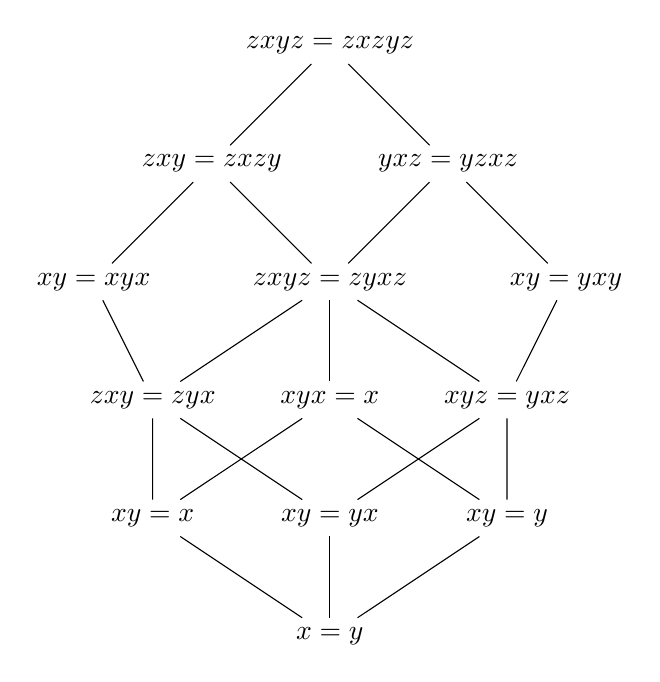
\begin{tikzpicture}[scale=1.5]
  \node (s1) at (0,0) {$zxyz=zxzyz$};
  
  \node (s2a) at (-1,-1) {$zxy=zxzy$};
  \node (s2b) at (1,-1) {$yxz=yzxz$};
  \draw (s1) to (s2a) {};
  \draw (s1) to (s2b) {};
  
  \node (s3a) at (-2,-2) {$xy=xyx$};
  \node (s3b) at (0,-2) {$zxyz=zyxz$};
  \node (s3c) at (2,-2) {$xy=yxy$};
  \draw (s2a) to (s3a) {};
  \draw (s2a) to (s3b) {};
  \draw (s2b) to (s3b) {};
  \draw (s2b) to (s3c) {};
  
  \node (s4a) at (-1.5,-3) {$zxy=zyx$};
  \node (s4b) at (0,-3) {$xyx=x$};
  \node (s4c) at (1.5,-3) {$xyz=yxz$};
  \draw (s3a) to (s4a) {};
  \draw (s3b) to (s4a) {};
  \draw (s3b) to (s4b) {};
  \draw (s3b) to (s4c) {};
  \draw (s3c) to (s4c) {};
  
  
  \node (s5a) at (-1.5,-4) {$xy=x$};
  \node (s5b) at (0,-4) {$xy=yx$};
  \node (s5c) at (1.5,-4) {$xy=y$};
  \draw (s4a) to (s5a) {};
  \draw (s4a) to (s5b) {};
  \draw (s4b) to (s5a) {};
  \draw (s4b) to (s5c) {};
  \draw (s4c) to (s5b) {};
  \draw (s4c) to (s5c) {};
  
  \node (s6) at (0,-5) {$x=y$};
  \draw (s5a) to (s6) {};
  \draw (s5b) to (s6) {};
  \draw (s5c) to (s6) {};
  
  %\node[thy,inner sep=.3cm,fill=gray] (t1) at (0,0) {};
  %\node at (t1.north west) {$S$};
  %\node at (t1) {$D$};
  %\node[thy,inner sep=.5cm,fill=lightgray] (s2) at (2,0) {};
  %\node[thy,inner sep=.3cm,fill=gray] (t2) at (2,0) {};
  %\node at (t2.north west) {$T$};
  %\node at (t2) {$C$};
  %\draw[view] (t1) to[out=10,in=170] node[above] {$\sigma$} (t2);
\end{tikzpicture}

%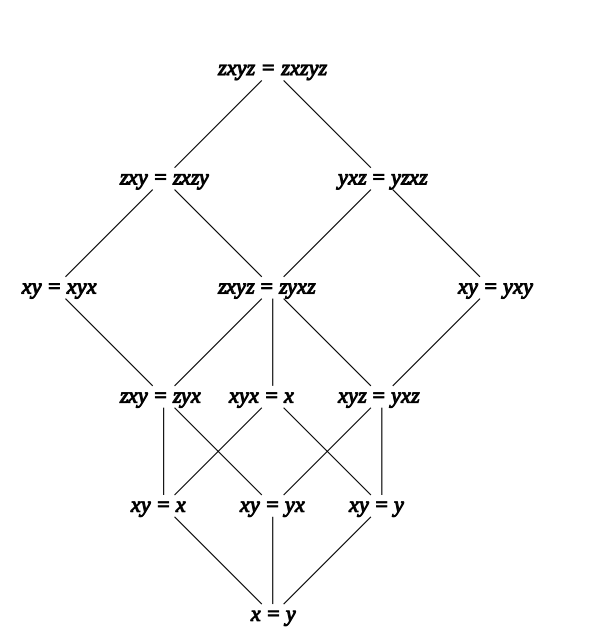
\includegraphics[width=0.6\textwidth]{bands}
\end{center}
\caption{The Lattice of Varieties of Bands}\label{fig:bands}
\end{figure}

%
%\begin{figure}
%\begin{tabular}{c|c}
%\begin{mmtcode}
%Band =
%  include ?SemiGroup
%  axiom_idemp : ⊦ ∀[x] x ∘ x ≐ x
%❚
%
%Regular =
%  include ?Band
%  axiom_regular : ⊦ ∀[x]∀[y]∀[z] 
%    z ∘ x ∘ z ∘ y ∘ z ≐ z ∘ x ∘ y ∘ z
%❚
%
%LeftNormal =
%  include ?Band
%  axiom_leftnormal : ⊦ ∀[x]∀[y]∀[z] 
%    z ∘ x ∘ z ∘ y ≐ z ∘ x ∘ y
%
%theory RightNormal =
%  include ?Band ❙
%  axiom_rightnormal : ⊦ ∀[x]∀[y]∀[z] 
%    y ∘ z ∘ x ∘ z ≐ y ∘ x ∘ z ❙ 
%❚
%
%theory Normal : ?Meta =
%  include ?Band ❙
%  axiom_normal :  ⊦ ∀[x]∀[y]∀[z] 
%    z ∘ x ∘ y ∘ z ≐ z ∘ y ∘ x ∘ z ❙
%❚
%\end{mmtcode} &
%\begin{mmtcode}
%implicit view Reg2LeftNormal : 
%    ?Regular -> ?LeftNormal =
%  include ?Band = ?Band ❙
%  axiom_regular = sketch "trivial" ❙
%❚
%
%implicit view Reg2RightNormal : 
%    ?Regular -> ?RightNormal =
%  include ?Band = ?Band ❙
%  axiom_regular = sketch "trivial" ❙
%❚
%
%implicit view LeftNormal2Normal : 
%    ?LeftNormal -> ?Normal =
%  include ?Band = ?Band ❙
%  axiom_leftnormal = sketch "trivial" ❙
%❚
%
%implicit view RightNormal2Normal : 
%    ?RightNormal -> ?Normal =
%  include ?Band = ?Band ❙
%  axiom_rightnormal = sketch "trivial" ❙
%❚
%\end{mmtcode}
%\end{tabular}
%
%\caption{Exemplary Theories for Some Varieties of Bands}\label{fig:bandsmmt}
%\end{figure}

%\section{Complex Theories and Morphisms}\label{sec:complex}
%We now add some complex theories and morphisms to \mmt.
\begin{grammar}
T      & \{\} \alt \bigcup\{\rep{T}\} \alt M(T)   & \text{complex theories}\\
M      & \{\} \alt \bigcup\{\rep{M}\} \alt M^T \alt M^T(M)   & \text{complex morphisms}
\end{grammar}

Their meanings are explained in the sequel.

\paragraph{Empty Theory}
The empty theory $\{\}\in\Thy$ and the empty morphism $\{\}\in\Mo{\{\}}{T}$ for $T\in\Thy$ are always well-formed.
Their semantics is given by $\flt{\{\}}=\es$ (in both cases).
$\{\}$ is an initial object in the category of theories.

The empty morphism is implicit.

\paragraph{Union of Theories}
For any finite set $\Theta\sq\Thy$ of theories, the union theory $\bigcup \Theta\in\Thy$ is always well-formed.
Its semantics is given by $\flt{(\bigcup\Theta)}=\bigcup_{T\in\Theta}\flt{T}$.
As special cases, we can recover $T\equiv\bigcup\{T\}$ and $\{\}\equiv\bigcup\es$.

We write $S\cup T$ for the binary union $\bigcup\{S,T\}$.
Binary union is a semi-lattice (with respect to $\harr$ and $\equiv$) with least element $\{\}$.

Clearly, we have $T\harr \bigcup\Theta$ if $T\in\Theta$.
Moreover, we define the include closure of a set of theories by $\cls{\Theta}=\{C|C\harr T, T\in\Theta\}$ (which is a topological closure operator).
Then we have $\bigcup Z\harr \bigcup \Theta$ iff $\cls{Z}\sq\cls{\Theta}$ and thus also $\bigcup Z\equiv \bigcup \Theta$ iff $\cls{Z}=\cls{\Theta}$.


Now consider morphisms $M_i\in\Mo{S_i}{T_i}$ for $i=1,\ldots,n$.
Let $\mu=\{M_1,\ldots,M_n\}$, $Z=\{S_1,\ldots,S_n\}$ and $\Theta=\{T_1,\ldots,T_n\}$.
The union morphism $\bigcup \mu: \bigcup Z \to \bigcup \Theta$ is well-formed if $M_i|_C\equiv M_j|_C$ whenever $C\harr S_i$ and $C\harr S_j$.
Its semantics is given by $\flt{(\bigcup \mu)}=\bigcup_{M\in\mu} \flt{M}$.

$\bigcup \mu$ is implicit if all $M_i$ are.

\paragraph{Pushout along Inclusion}
For morphisms $M\in\Mo{S}{T}$ and $S\harr X$, the pushout $T\harr M(X)$ with the morphism $M^X\in\Mo{X}{M(X)}$ are well-formed if for all $C\harr X$ and $C\harr T$ also $C\harr S$.

In that case, for $u\in\Mo{T}{U}$ and $x\in\Mo{X}{U}$, the universal morphism $M^u(x)\in\Mo{M(X)}{U}$ of the pushout is well-formed if $x|_S\equiv M;u$.

Their semantics is defined by
\[\flt{M(X)}=\flt{T}\cup \{c[:M(t)][=M(d)]\;|\;c[:t][=d]\in\flt{X}\sm\flt{S}\}\]
\[\flt{(M^X)}=\flt{M}\cup\{c:=c\;|\;c\in\dom{X}\sm\dom{S}\}\]
\[\flt{M^u(x)}=\flt{u}\cup\{c:=x(c)\;|\;c\in\dom{X}\sm\dom{S}\}\]

Note that our definition of $\flt{m(X)}$ crucially exploits the condition that $\dom{X}\sm\dom{S}$ and $\dom{T}$ must be disjoint.
Thus, we obtain $\dom{X}\sm\dom{S}\sq\dom{m(X)}$ and $m^X$ maps these identifiers to themselves.

%(Note that if $M$ is implicit, then necessarily $m|_C\equiv\id{C}$.)

$m^X$ is implicit if $m$ is.\ednote{Can this always be implicit? Even if it can, it is probably not desirable. Compare left-/right-neutral element.}
\ednote{Should there be implicit extensions of morphism? E.g., $m^X$ could be implicit relative to $m$, i.e., we write $m$ and it is inferred as $m^X$. Does that yield canonical structures?}
$m^u(x)$ is implicit if $m$ and $u$ are.


%Pushouts are coherent:
%  $(m;n)(X)\equiv n(m(X))$ if the right hand side is defined.
%  If $X\harr Y$, then $m(X)\harr m(Y)$ if $m(Y)$ is defined.
%  $\id{S}(X)\equiv X$ (always defined).
%  $m(S)\equiv S$ (always defined).
%  
%Pushout over the empty morphism is defined iff $X$ and $T$ are disjoint.
%In that case, it is the union. (But not all unions arise in this way.)
%
%Pushout distributes over union:
%  $m(X\cup Y)\equiv m(X)\cup m(Y)$ (equi-defined)
%  $m^{X\cup Y}\equiv m^X\cup m^Y$ (?)
%  
%  does not make sense:
%  $(\bigcup m_i)(X)\equiv \bigcup \{m_i(X)\}$ 
%  $(\bigcup m_i)^X\equiv \bigcup\{m_i^X\}$
%

% Theorem: For every theory $T$, we have $\dom{T}=\dom{t_1}\cup\ldots\cup\dom{t_n}$ for atomic theories $t_i$.


\section{Related Work}
\subsection{Realms}

\cite{realms} defines a realm (essentially) as a certain cluster of theories:
\begin{compactitem}
\item a set of isomorphic theories $B_1,\ldots,$
\item for each $B_i$, a set of retractable extensions $E^i_1,\ldots,$
\item a theory $F$ including all of the above.
\end{compactitem}
The intuition is that the $B_i$ are alternative definitions of a theory; the $E^i_j$ add definitions and theorems; and $F$ aggregates everything into the outwardly visible interface (the face) of the realm.

A good example is the realm of topological spaces with the $B_i$ corresponding to the various possible definitions (via neighborhoods, open sets, closure operator, etc.).

Users of the realm include only the face and thus (i) gain access to all derived knowledge in the theory of topological spaces, and (ii) do not have to commit to one particular definition.
Indeed, this corresponds more closely to the way how conventional mathematics sees the theory of topological spaces.

\cite{realms} calls for an implementation of realms as a new primitive concept in addition to theories and morphisms.
However, in the presence of implicit morphisms, we do not need it: All we have to do is to designate the isomorphisms and the retraction is implicit and include any one of the $B_i$ into $F$.


\subsection{Canonical Structures in Coq}

\cite{gonthier_packaging}


\subsection{Implicit Conversions in Scala}

The Scala programming language \cite{scala} has a clean implementation of implicit conversions between any two types.
If we think of functions between classes as theory morphisms, this corresponds to implicit theory morphisms.

Contrary to \mmt, a conversion is only available if explicitly imported into the current namespace.
Moreover, Scala does not chain conversions, i.e, the composition of implicit morphisms is not implicit.
Scala's limitations are intentional: Their goal is to prevent programmers from overusing implicit conversions because that can be very confusing to readers.

These limitations are lifted in \mmt's conversions can only act between theories anyway.
Thus, their potential to confuse is smaller.
Moreover, the use of qualified identifiers in \mmt means that readers can always tell where an identifier is implicitly-included from, and the \mmt IDE can always show the implicit morphism along which it is imported.

\ednote{drawback: global data structure}

\section{Conclusion}
\paragraph{Implicit Conversions}
The need for implicit conversions has been recognized in many formal systems.
In all cases, similar uniqueness constraints are employed as in ours.

\textbf{Type-level} conversions are functions between types such as the conversion from natural numbers to integers.
\textbf{Theory-level} conversions are morphisms between theories, like in this paper, or similar constructs.
The latter can be seen as a special case of the former: if every theory is seen as the type of its models (as in \cite{MRK:modelsof:18}), then reduction along an implicit morphism $S\to T$ induces a conversion from $T$-models to $S$-models.
Type-level conversions are present in many systems, e.g., the Coq proof assistant \cite{coq} or the Scala programming language.
%In both cases, this includes theory-level conversions between the respective analogues of theories
The novelty in our approach is to restrict conversions two-fold: firstly to the theory level, secondly to those conversion functions that can be expressed as theory morphisms.
This significantly reduces the complexity and permits an elegant logic-independent semantics, while still being practically useful.

Some formal systems support theory-level conversions without explicitly using theory morphisms.
This is common in systems that use type classes as an analogue to theories.
For example, the \texttt{sublocale} declarations of the proof assistant Isabelle \cite{isabelle_locales} or the \texttt{deriving} declarations of the programming language Haskell can be seen as implicit morphisms even though no primitive concept of morphism objects is employed.
Our implicit morphisms yield a simpler and more expressive theory-level conversion system at the price of having an additional primitive concept.
% Löh paper on deriving via not published yet
%\cite{gonthier_packaging}

\paragraph{Structuring Theories}
In systems that maintain large diagrams of theories, the problems solved by our approach have been recognized for some time.
For example, the IMPS system \cite{imps} allowed using theory morphisms to retroactively add defined constants to a previously declared theory.
This corresponds to a definitional extension with an implicit retraction morphism as in Sect.~\ref{sec:inverse}.

In \cite{realms}, the idea of \emph{realms} was introduced as a way to bundle a set of isomorphic theories and their definitional extensions into a single interface.
The paper called for an implementation of realms as a new primitive concept in addition to theories and morphisms.
In contrast, the much simpler feature of implicit morphisms achieves very similar goals: realms can be recovered by marking all isomorphisms as \emph{implicit} and all extensions as \emph{definitional}.

%\begin{compactitem}
%\item a set of isomorphic theories $B_1,\ldots,$
%\item for each $B_i$, a set of retractable extensions $E^i_1,\ldots,$
%\item a theory $F$ including all of the above.
%\end{compactitem}
%The intuition is that the $B_i$ are alternative definitions of a theory; the $E^i_j$ add definitions and theorems; and $F$ aggregates everything into the outwardly visible interface (the face) of the realm.
%A good example is the realm of topological spaces with the $B_i$ corresponding to the various possible definitions (via neighborhoods, open sets, closure operator, etc.).
%
%Users of the realm include only the face and thus (i) gain access to all derived knowledge in the theory of topological spaces, and (ii) do not have to commit to one particular definition.
%Indeed, this corresponds more closely to the way how conventional mathematics sees the theory of topological spaces.

\paragraph{Scalability and Scoping}
Future work will focus on utilizing and evaluating implicit morphisms in large libraries, i.e., diagrams with thousands of theories and as many implicit morphisms as possible.

In doing so, we will pay particular attention to some problems that implicit conversions can cause at large scale.
Users can be confused when implicit conversions are applied that they are not aware of, and different users may also have different preferences for which conversions should be implicit.
Moreover, critically, different developments may be incompatible if they introduce different implicit morphisms between the same theories.
For those reasons, Scala, for example, only applies implicit conversions that are imported into the current namespace.

We anticipate that these problems will lead to an evolution of our solution that allows more localized control over which morphisms are implicit.
Thus, instead of a single global diagram of implicit morphisms, every context may carry its own local one.
But we defer this until the current implementation has been used to conduct very large case studies.

%Moreover, the use of qualified identifiers in \mmt means that readers can always tell where an identifier is implicitly-included from, and the \mmt IDE can always show the implicit morphism along which it is imported.




\bibliographystyle{alpha}
\bibliography{../../../../frabe/Program_Data/Latex/bib/rabe,../../../../frabe/Program_Data/Latex/bib/systems,../../../../frabe/Program_Data/Latex/bib/institutions,../../../../frabe/Program_Data/Latex/bib/pub_rabe,../../../../frabe/Program_Data/Latex/bib/historical}

\end{document}